% Options for packages loaded elsewhere
\PassOptionsToPackage{unicode}{hyperref}
\PassOptionsToPackage{hyphens}{url}
\PassOptionsToPackage{dvipsnames,svgnames,x11names}{xcolor}
%
\documentclass[
  letterpaper,
  DIV=11,
  numbers=noendperiod]{scrartcl}

\usepackage{amsmath,amssymb}
\usepackage{iftex}
\ifPDFTeX
  \usepackage[T1]{fontenc}
  \usepackage[utf8]{inputenc}
  \usepackage{textcomp} % provide euro and other symbols
\else % if luatex or xetex
  \usepackage{unicode-math}
  \defaultfontfeatures{Scale=MatchLowercase}
  \defaultfontfeatures[\rmfamily]{Ligatures=TeX,Scale=1}
\fi
\usepackage{lmodern}
\ifPDFTeX\else  
    % xetex/luatex font selection
\fi
% Use upquote if available, for straight quotes in verbatim environments
\IfFileExists{upquote.sty}{\usepackage{upquote}}{}
\IfFileExists{microtype.sty}{% use microtype if available
  \usepackage[]{microtype}
  \UseMicrotypeSet[protrusion]{basicmath} % disable protrusion for tt fonts
}{}
\makeatletter
\@ifundefined{KOMAClassName}{% if non-KOMA class
  \IfFileExists{parskip.sty}{%
    \usepackage{parskip}
  }{% else
    \setlength{\parindent}{0pt}
    \setlength{\parskip}{6pt plus 2pt minus 1pt}}
}{% if KOMA class
  \KOMAoptions{parskip=half}}
\makeatother
\usepackage{xcolor}
\setlength{\emergencystretch}{3em} % prevent overfull lines
\setcounter{secnumdepth}{-\maxdimen} % remove section numbering
% Make \paragraph and \subparagraph free-standing
\ifx\paragraph\undefined\else
  \let\oldparagraph\paragraph
  \renewcommand{\paragraph}[1]{\oldparagraph{#1}\mbox{}}
\fi
\ifx\subparagraph\undefined\else
  \let\oldsubparagraph\subparagraph
  \renewcommand{\subparagraph}[1]{\oldsubparagraph{#1}\mbox{}}
\fi


\providecommand{\tightlist}{%
  \setlength{\itemsep}{0pt}\setlength{\parskip}{0pt}}\usepackage{longtable,booktabs,array}
\usepackage{calc} % for calculating minipage widths
% Correct order of tables after \paragraph or \subparagraph
\usepackage{etoolbox}
\makeatletter
\patchcmd\longtable{\par}{\if@noskipsec\mbox{}\fi\par}{}{}
\makeatother
% Allow footnotes in longtable head/foot
\IfFileExists{footnotehyper.sty}{\usepackage{footnotehyper}}{\usepackage{footnote}}
\makesavenoteenv{longtable}
\usepackage{graphicx}
\makeatletter
\def\maxwidth{\ifdim\Gin@nat@width>\linewidth\linewidth\else\Gin@nat@width\fi}
\def\maxheight{\ifdim\Gin@nat@height>\textheight\textheight\else\Gin@nat@height\fi}
\makeatother
% Scale images if necessary, so that they will not overflow the page
% margins by default, and it is still possible to overwrite the defaults
% using explicit options in \includegraphics[width, height, ...]{}
\setkeys{Gin}{width=\maxwidth,height=\maxheight,keepaspectratio}
% Set default figure placement to htbp
\makeatletter
\def\fps@figure{htbp}
\makeatother

\KOMAoption{captions}{tableheading}
\makeatletter
\@ifpackageloaded{caption}{}{\usepackage{caption}}
\AtBeginDocument{%
\ifdefined\contentsname
  \renewcommand*\contentsname{Table of contents}
\else
  \newcommand\contentsname{Table of contents}
\fi
\ifdefined\listfigurename
  \renewcommand*\listfigurename{List of Figures}
\else
  \newcommand\listfigurename{List of Figures}
\fi
\ifdefined\listtablename
  \renewcommand*\listtablename{List of Tables}
\else
  \newcommand\listtablename{List of Tables}
\fi
\ifdefined\figurename
  \renewcommand*\figurename{Figure}
\else
  \newcommand\figurename{Figure}
\fi
\ifdefined\tablename
  \renewcommand*\tablename{Table}
\else
  \newcommand\tablename{Table}
\fi
}
\@ifpackageloaded{float}{}{\usepackage{float}}
\floatstyle{ruled}
\@ifundefined{c@chapter}{\newfloat{codelisting}{h}{lop}}{\newfloat{codelisting}{h}{lop}[chapter]}
\floatname{codelisting}{Listing}
\newcommand*\listoflistings{\listof{codelisting}{List of Listings}}
\makeatother
\makeatletter
\makeatother
\makeatletter
\@ifpackageloaded{caption}{}{\usepackage{caption}}
\@ifpackageloaded{subcaption}{}{\usepackage{subcaption}}
\makeatother
\ifLuaTeX
  \usepackage{selnolig}  % disable illegal ligatures
\fi
\usepackage{bookmark}

\IfFileExists{xurl.sty}{\usepackage{xurl}}{} % add URL line breaks if available
\urlstyle{same} % disable monospaced font for URLs
\hypersetup{
  pdftitle={Reciprocal relationships, reverse causality, and temporal ordering: Testing theories with cross-lagged panel models},
  pdfauthor={Charles C. Lanfear; Thiago R. Oliveira},
  colorlinks=true,
  linkcolor={blue},
  filecolor={Maroon},
  citecolor={Blue},
  urlcolor={Blue},
  pdfcreator={LaTeX via pandoc}}

\title{Reciprocal relationships, reverse causality, and temporal
ordering: Testing theories with cross-lagged panel models}
\author{Charles C. Lanfear \and Thiago R. Oliveira}
\date{}

\begin{document}
\maketitle

\begin{quote}
Abstract from panel; we may want to decide on specific illustrative case
after we've laid out framework of paper, as we want our case to exhibit
every potential issue.
\end{quote}

Reciprocal causal relationships are a common feature of criminological
theories. For example, police forces tend to use force more often in
areas where crime concentrates, while at the same time legal cynicism
theory suggests that cumulative exposures to police use-of-force can
foster criminal activity. When multiple observations over time are
available, cross-lagged panel models are commonly used to estimate these
reciprocal effects. This is often done without careful attention to the
assumptions that must be satisfied to produce valid estimates, such as
correctly specified temporal lags, sufficient inter-temporal variation,
and proper accounting for unobserved heterogeneity. Failure to satisfy
these assumptions can produce severe issues including spurious
associations and parameter estimates that are biased or even reversed in
direction. In addition, reciprocal relationships violate causal
assumptions based on graphical tools; criminological theories that
suggest reciprocal causal relationships usually have an underlying
macro-micro mechanism often not accounted for in empirical models. We
provide guidance on how to align theory, model specification, and choice
of estimator and illustrate this using an empirical example. We use data
from Chicago at the census tract level and model the potential
reciprocal relationship between police use-of-force and violent crime
between 2004 and 2016. We finalise highlighting the importance of
criminological theory and careful attention to empirical implications of
theoretical premises when investigating reciprocal relationships

\section{Introduction}\label{introduction}

\begin{itemize}
\tightlist
\item
  When do we expect reciprocal effects?

  \begin{itemize}
  \tightlist
  \item
    What are reciprocal effects \emph{really}?
  \item
    Separate theoretical and methodological concerns
  \end{itemize}
\item
  What must a model do to capture these?
\item
  Use 3 wave model as example
\item
  Might be worth taking a clear but extremely concise perspective on
  causality to ward off pedants
\item
  Terminology

  \begin{itemize}
  \tightlist
  \item
    Strict exogeneity
  \item
    Predetermined regressors (weakly exogenous, sequentially exogenous)
  \end{itemize}
\item
  Explanation of how what we're doing is different from recent reviews
  of CLPM literature, e.g., Zyphur et al.~(2020).

  \begin{itemize}
  \tightlist
  \item
    Zyphur et al.~elaborate a complete generalized cross-lagged panel
    model that accounts for a wider range of specifications. Here we
    focus on key problems that appear in applied literature.
  \end{itemize}
\end{itemize}

\begin{quote}
Thiago: I think that sounds great. I've always pictured this as going
deep in the ``what are reciprocal effects \emph{really}?'' question. The
way I see it is the following. DAGs do not allow for reciprocal effects.
Yet, lots of theories loosely suggest reciprocal effects. Some people
suggest that this might be a limitation of causal graphs (need to find
references for this). But I don't think it's a limitation of causal
graphs at all, instead I think it's limitation in how we commonly
translate theories into causal graphs. It is possible (even probable?)
that all criminological theories that suggest reciprocal relationships
are actually correct, but they're missing a crucial component: time. At
close inspection, theories don't suggest that X causes Y and Y causes X
simultaneously; they probably suggest that, in a very simple form, past
X causes future Y and that past Y causes future X---and variations of
that. So, one thing we can include here is the role of time in
translating theories into DAGs---and, in doing so, more deeply
discussing what reciprocal effects really are.
\end{quote}

\begin{quote}
Thiago: I understand this rules out reciprocal simultaneous effects. I'm
still not convinced those make sense theoretically (and even
statistically, as per Allison).
\end{quote}

\section{Notation and diagrams}\label{notation-and-diagrams}

We should be specific and consistent in choosing graphical
representations and notation.

DAGs are easy to understand but rule out contemporaneous reciprocal
relationships. This is good in one respect, as causal effects are always
time ordered. Perhaps we separate causal models from statistical models
explicitly by using DAGs for causal models and SEM path diagrams for
statistical models. Then using that, we talk about situations under
which modeling something as contemporaneous is necessary.

Relatedly, something I've never seen done is using DAGs to really
elaborate how we should think about waves of panel data as snapshots
during temporal processes. For example, you might imagine a causal
process like that below where we only observe at times 1, 3, and 5
despite the process operating over 1 unit lags. This is a
discretization, of course, and you can imagine many processes are
essentially continuous with hundreds of steps in between observations.

\begin{quote}
In below diagrams, I'd prob make the observed ones x1, x2, x3, y1, y2,
y3 and intervening ones something else, e.g., x1.5
\end{quote}

\begin{figure}

\centering{

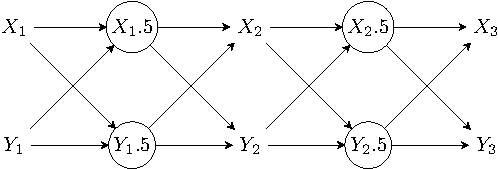
\includegraphics{jdlcc_clpm_draft_files/figure-pdf/fig-2-theory-dag-1.pdf}

}

\caption{\label{fig-2-theory-dag}Directed acyclic graph representation
of CLPM}

\end{figure}%

\begin{figure}

\centering{

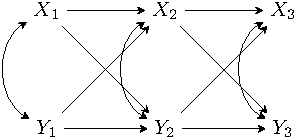
\includegraphics{jdlcc_clpm_draft_files/figure-pdf/fig-3-estimation-1.pdf}

}

\caption{\label{fig-3-estimation}SEM path diagram representation of
CLPM}

\end{figure}%

\begin{itemize}
\tightlist
\item
  DAGs for theory, SEM path diagrams for estimation?
\end{itemize}

\begin{quote}
Thiago: Yes, that makes sense, but I think we should make the effort to
make them consistent. That is, the structural part of the SEM should
also be a DAG. Thiago: Bollen \& Pearl 2009 provide a nice discussion
about the notational relationship between SEM path diagrams and DAGs.We
should also look at Imai \& Kim's three papers on causal inference with
panel data. They use DAGs and they're so well written. I don't think
they discuss reciprocal effects at all (could be wrong), but we could
rely on them from a notational point of view in using DAGs to depict
temporal processes.
\end{quote}

\section{Motivating example}\label{motivating-example}

\begin{quote}
We've written up ESC using legal cynicism as motivating example, but if
we find it to be too complicated, we could also use the Airbnb paper for
ESC (doesn't make sense for JDLCC though). It is nice because it has a
DAG to motivate an estimation strategy with contemporaneous effects:
\end{quote}

\begin{figure}[H]

{\centering 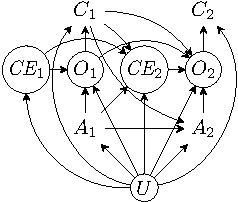
\includegraphics{jdlcc_clpm_draft_files/figure-pdf/airbnb-1-1.pdf}

}

\caption{Theoretical model. CE is collective efficacy, O is criminal
opportunity, C is crime, A is short-term lettings, U is omitted
confounders}

\end{figure}%

\begin{figure}[H]

{\centering 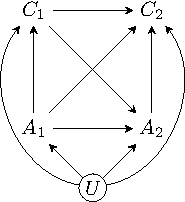
\includegraphics{jdlcc_clpm_draft_files/figure-pdf/airbnb-2-1.pdf}

}

\caption{Estimation model. C is crime, A is short-term lettings, U is
omitted time- and unit-specific confounders}

\end{figure}%

Alternatively, we might select something with ambiguous contemporaneous
directionality to motivate different estimation approaches, e.g., the
Vaisey \& Miles both effects approach or the Allison unanalyzed
correlation approach.

\begin{quote}
Yes, I agree that LC could be too complicated for this because it's an
obvious story about reciprocal relationships. For ESC, we should just go
with whatever's easier. But for JDLCC, I feel like we should pick
something (preferably at the individual level as it's JDLCC) that is
intuitively and obviously reciprocal. Can't figure out what yet, though.
\end{quote}

\section{Issue 1: Temporal Order}\label{issue-1-temporal-order}

\begin{itemize}
\tightlist
\item
  Unusual form of bias as documented by Vaisey \& Miles that can flip
  signs:

  \begin{itemize}
  \tightlist
  \item
    If true model is \(y = \beta x_t + \alpha_i + e_{it}\) and you fit
    \(y = \beta^* x_{t-t} + \alpha_i + e_{it}\),
    \(E(\beta^*) = -0.5\beta\), i.e., as
    \href{https://statisticalhorizons.com/getting-the-lags-right-a-new-solution/}{Allison
    (2022)} says ``a positive contemporaneous effect of \(x\) gets
    transformed into an artifactually negative lagged effect''.
  \end{itemize}
\item
  Probably the most underappreciated issue as it may produce misleading
  results that reject or overturn theories

  \begin{itemize}
  \tightlist
  \item
    Papers that find negative effects when theory suggests positive ones
    may be the result of this bias.
  \end{itemize}
\end{itemize}

\subsection{Solutions}\label{solutions}

\begin{itemize}
\tightlist
\item
  Theoretical ideal: Get it right
\item
  Vaisey \& Miles: Do both lagged and contemporaneous

  \begin{itemize}
  \tightlist
  \item
    If no contemporaneous effect, only lagged, you're probably fine. If
    contemporaneous shows up, you can't definitively determine direction
    of contemporaneous effect.
  \end{itemize}
\item
  Allison: Partial correlation model with lagged effect and
  contemporaneous residual covariance

  \begin{itemize}
  \tightlist
  \item
    This is least biased approach if parameter of interest is
    \(\beta x_{t-1}\), but cannot estimate \(\beta x_{t}\)
  \item
    This still does not adjudicate between direction of contemporaneous
    effects; if effect is entirely contemporaneous, all relationship
    will be in residual covariance.
  \end{itemize}
\end{itemize}

\begin{figure}[H]

{\centering 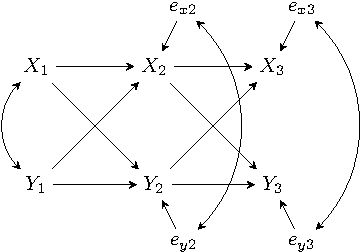
\includegraphics{jdlcc_clpm_draft_files/figure-pdf/allison-2022-1.pdf}

}

\caption{Allison (2022) recommendation}

\end{figure}%

\section{Issue 2: Unobserved
heterogeneity}\label{issue-2-unobserved-heterogeneity}

\begin{itemize}
\tightlist
\item
  Probably the most commonly encountered issue
\item
  Might also raise treatment heterogeneity here as different but related
  issue not as easily addressed in CLPMs as in TWFE

  \begin{itemize}
  \tightlist
  \item
    Exception is time-specific treatment heterogeneity which is easily
    permitted by allowing wave-specific parameters as in Allison's model
  \item
    A potentially useful application for wave-specific parameters is
    when you have unevenly spaced data; I think latent growth models
    would get at his too but I'm not very familiar with them.
  \end{itemize}
\end{itemize}

\subsection{Solutions}\label{solutions-1}

\begin{itemize}
\tightlist
\item
  RI-CLPM and related approaches

  \begin{itemize}
  \tightlist
  \item
    These are correlated stable trait models; I'm not very familiar
  \item
    Seems to address time stable unit heterogeneity
  \end{itemize}
\item
  Allison's FE dynamic panel model

  \begin{itemize}
  \tightlist
  \item
    Can handle both under same assumptions and problems
  \item
    Allison's ML-SEM approach is related to this Mundlak model; augments
    it with predetermined regressors.
  \end{itemize}
\end{itemize}

\begin{quote}
Thiago: I think the RI-CLPM is equivalent to Allison's FE DPM when it
comes to handling unobserved heterogeneity, but need to check it out
more closely.
\end{quote}

\section{Issue 3: Inter-temporal
variation}\label{issue-3-inter-temporal-variation}

\begin{itemize}
\tightlist
\item
  Maybe show some illustrative math here to show that
  \(Var(Y_2|Y_1) \rightarrow 0\) as \(\rho(Y_1,Y_2) \rightarrow 1\)
  approaches 1; i.e., you rapidly run out of anything to explain.

  \begin{itemize}
  \tightlist
  \item
    This is essentially a multicollinearity problem: Unbiased and
    consistent but high variance in estimates makes any particular
    estimate suspect.
  \end{itemize}
\item
  Rarely appreciated outside time series literature but common when
  waves are narrowly spaced
\item
  With random measurement error, the error becomes proportionally larger
  as time periods get narrower

  \begin{itemize}
  \tightlist
  \item
    May mean you can address in part with measurement models
  \item
    Note the endogenous variables are regressors, so measurement error
    biases parameter estimates as well
  \end{itemize}
\end{itemize}

\subsection{Solutions}\label{solutions-2}

\begin{itemize}
\tightlist
\item
  This is first and foremost a data problem, so you want to attack it
  during design of data collection if possible

  \begin{itemize}
  \tightlist
  \item
    Sample to maximize change
  \item
    Look for shocks
  \end{itemize}
\item
  If you can't collect new data, look at different aggregations or wave
  skips

  \begin{itemize}
  \tightlist
  \item
    Small change at a large unit may mask larger changes in small units
  \item
    Should prob only consider skipping waves if it makes sense
    theoretically and/or you're facing serious empirical
    underidentification problems.
  \end{itemize}
\end{itemize}

\section{General Advice}\label{general-advice}

\begin{itemize}
\tightlist
\item
  Allison's FE model should prob be the default as it is most robust
\end{itemize}

\section{Conclusion}\label{conclusion}

\begin{quote}
Thiago: Sounds great!
\end{quote}



\end{document}
